\chapter[2024 June]{June 2024}

\section{June Schedule}

\TabRef{tab:schedule_06} Shows the EPR 402 schedule for June 2024.
\begin{table}[H]
  \centering
  \caption{EPR 402 Schedule for June 2024}
  \label{tab:schedule_06}
    \begin{tabular}{ !{\vrule width 1.1pt}
                    c!{\vrule width 1pt}
                    c!{\vrule width 1pt}
                    c!{\vrule width 1pt}
                    p{8.6cm}!{\vrule width 1pt}}
    \noalign{\hrule height 1pt}
    \cellcolor[gray]{0.9} \textbf{Week} &
    \cellcolor[gray]{0.9} \textbf{Date} &
    \cellcolor[gray]{0.9} \textbf{Part} &
    \cellcolor[gray]{0.9} \textbf{Required reading / Assignment due date }
    \\ \noalign{\hrule height 1pt}
    13     &  3 Jun --   7 Jun & 2 &
    \begin{itemize}
        \item Baseline trainer
        \item Use TensorFlow
    \end{itemize}
    \\ \hline
    14     &  10 Jun --   14 Jun & 3 &
    \begin{itemize}
        \item Obtain embedded device
        \item Transfer code to embedded device
    \end{itemize}
    \\ \hline
       &  17 Jun --   21 Jun &   & Exam
    \\ \hline
    15     &  24 Jun --   28 Jun & 3 &
    \begin{itemize}
        \item Ensure all libraries are installed
        \item Debug code on embedded device
    \end{itemize}
    \\ \hline
    \end{tabular}
\end{table}

% \subsection{Practical 3}
% Started design of AAF. Using too large resistor values reduce the cut-off frequency. Using unity gain Sallen-key configuration:
% \begin{figure}[H] 
% \centering
%     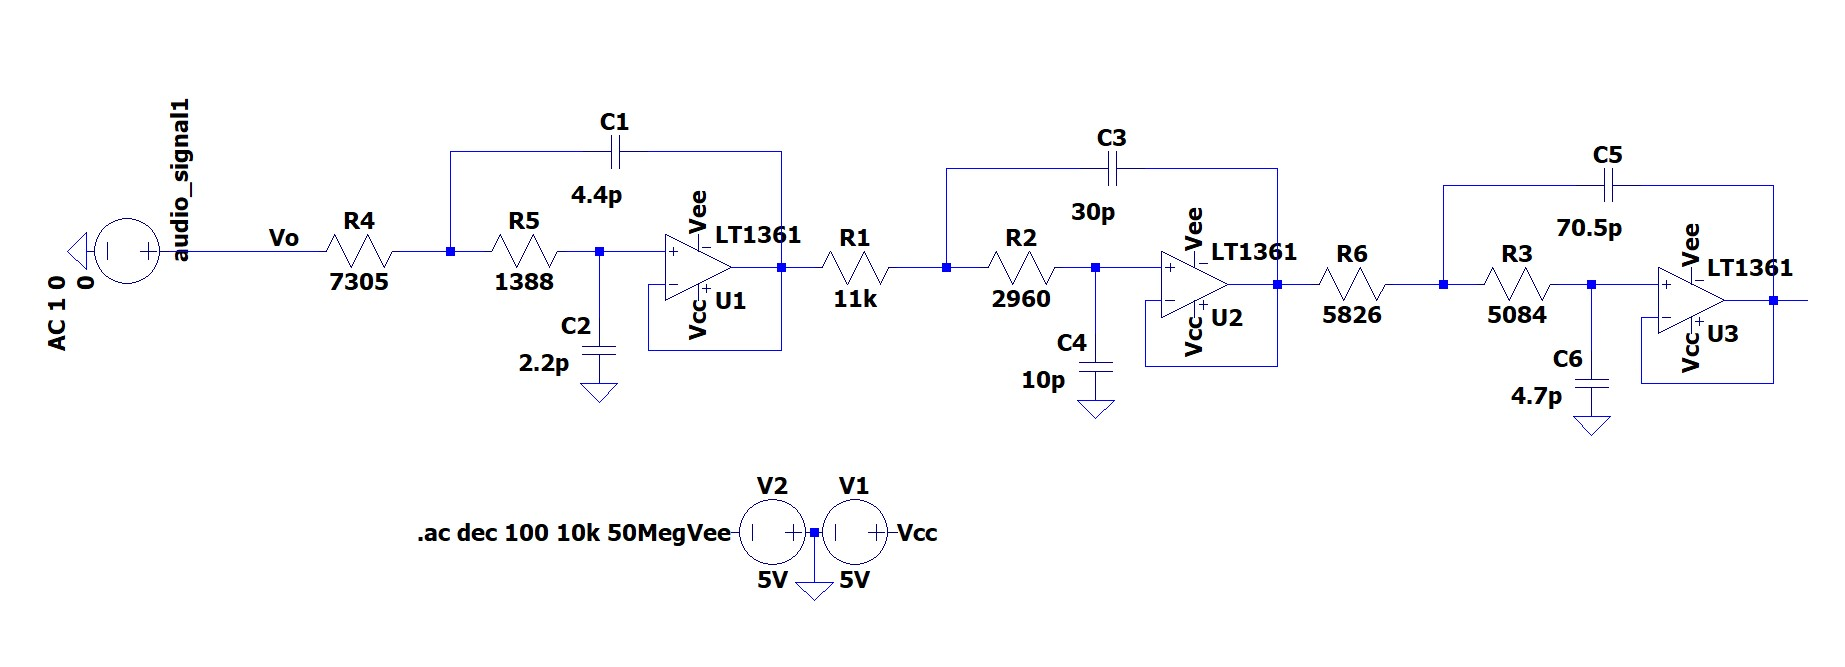
\includegraphics[width=0.8\textwidth]{2021/Images/Simulation/butterworth6thOrder.jpg} 
%   \caption{$6^{th}$ order butterworth AAF Circuit}
%   \label{fig:outputsignalFreq2}
% \end{figure}

%   \begin{figure}[H] 
% \centering
%     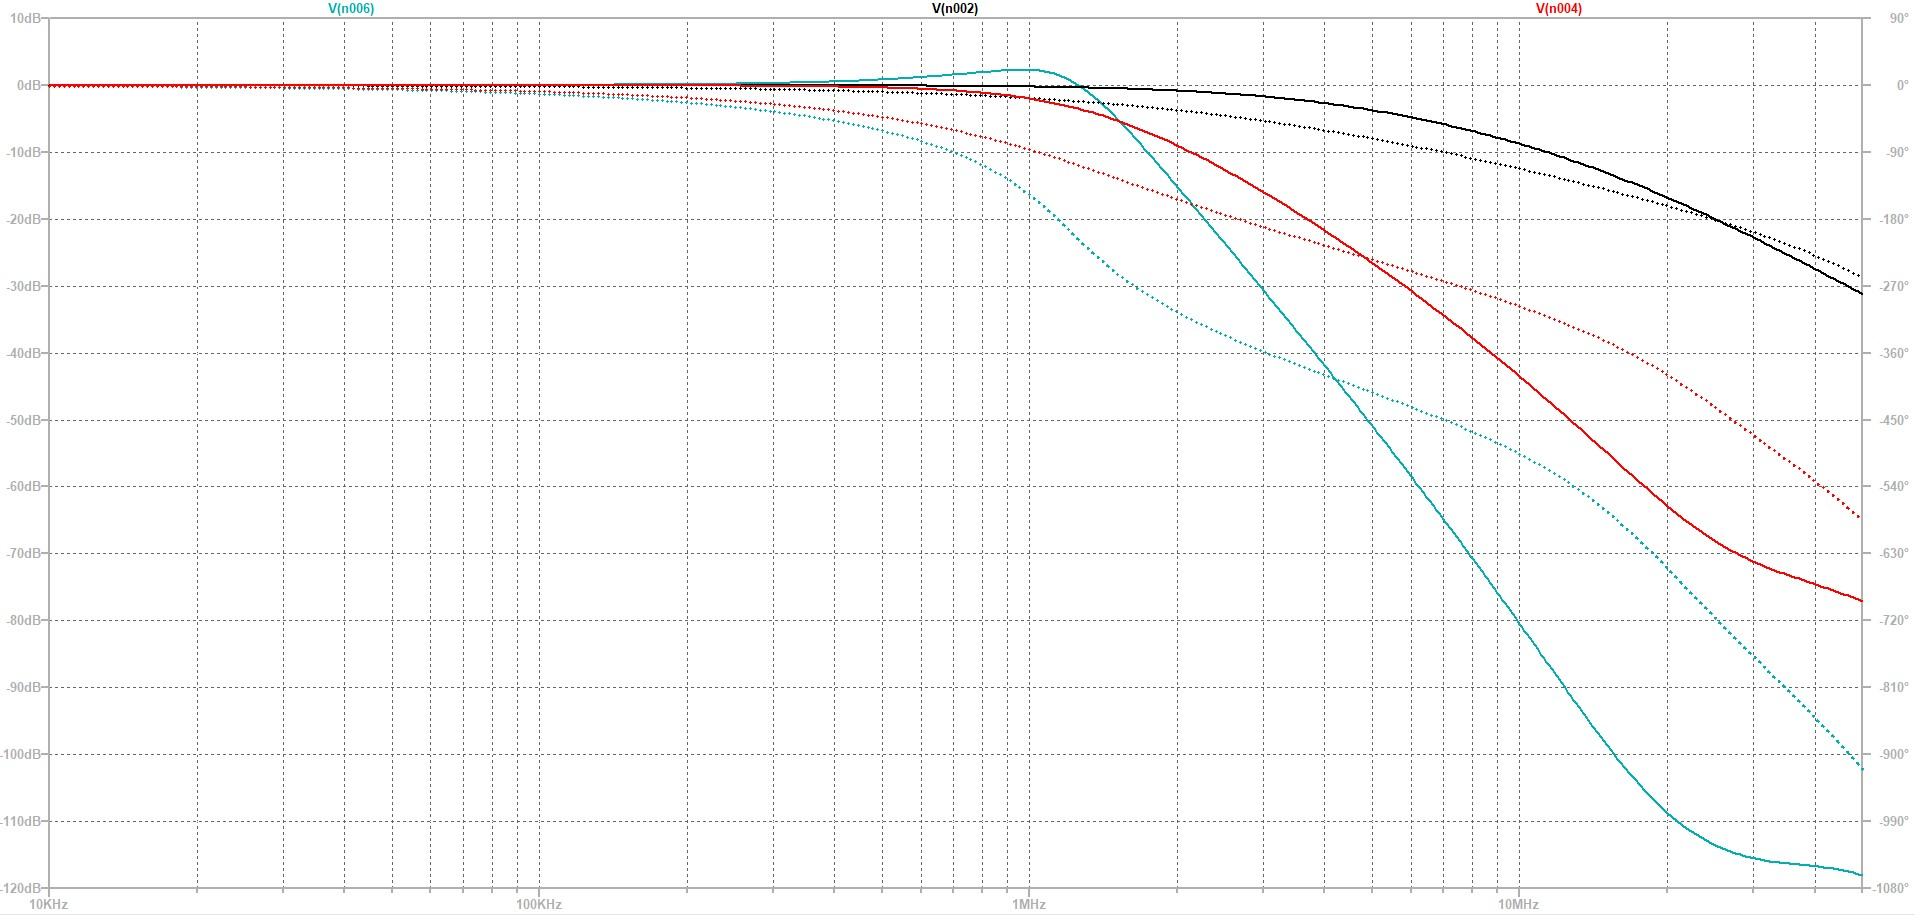
\includegraphics[width=0.8\textwidth]{2021/Images/Simulation/butterworth6thOrderResponse.jpg} 
%   \caption{$6^{th}$ order butterworth AAF Circuit}
%   \label{fig:outputsignalFreq2}
% \end{figure}
% As seen above the filter response create a ripple close to the cut-off frequency, this will need to be adjusted. As well as the cut-off frequency being $1.42MHz$ at the moment. 

% \pendsign

% \section[2021/06/17]{Thursday, 17 June 2021}
% \subsection{ADC}
% The STM32F429 Discovery Board contains three 12-bit ADCs. A single ADC can sample up to $2.4MSPS$, dual interleaved up to $4.8MSPS$ and triple interleaved up to $7.2MSPS$. The upper frequency of the AM band is $1.6065MHz$, sampling at or above $2 \times f_c = 3.213MHz$, thus dual interleaved ADC sampling will be adequate.
% \begin{align}
%     Step Size &= \frac{V_{ref}}{2^n} \\
%     &= \frac{3.6}{2^{12}} \\
%     &= 0.8789mV
% \end{align}

% Using dual interleaved ADCs will allow the one to sample the data while the other is busy with conversion. Thus doubling the effective frequency of sampling. 

% \subsection{Sampling}
% The minimum frequency resolution $= 3kHz$ thus, there need to be 360 bins. 

% \subsection{Low-pass filter}
% The low-pass filter will be used after the \ac{DAC}, to remove any irregularities from the signal created in the Digital to Analog conversion. The cut-off frequency $= 4.5kHz$, because that is the theoretical maximum audio bandwidth \cite{AMspectrumSidebands}. A simple $2^{nd}$ or $4^{th}$ order Butterworth filter will suffice.


% \subsection{Digital bandpass filter}
% The out of band emissions need to adhere to the following standards:
% \begin{align}
%     \pm 0.5F &= 0dB \\
%     \pm 0.7F &= 35dB \\
%     \pm 2.95F &= 60dB
% \end{align}

% \pendsign

% \section[2021/06/18]{Friday, 18 June 2021}
% \subsection{ADC \& Sampling}
% The maximum sampling frequency a single ADC on STM32F45K22 can achieve is $2.4MSPS$, the required sampling frequency, based on Nyquist theorem, is $3.213MHz$ thus dual interleaved mode will be used with the ADCs sampling at $2.4MSPS$ to achieve $F_s = 4.8MHz$. Each ADC is configured to have a minimum sampling rate of $2.4MSPS$, with $f_{ADC} = 36MHz$. $T_s$ is the sampling time given in ADC cycles, with $T_{conv} = 12 cycles$ \cite{STM32ADC}.

% \begin{align}
%     T_s &= \frac{f_{ADC}}{F_s} - 12.5 \\
%     &= \frac{42\times 10^{6}}{2.4\times 10^{6}} - 12 \\
%     &= 3
% \end{align}
% \begin{align}
%     T_{rate} &= T_s + T_{conv} \\
%     &= 15 \quad \text{cycles} \\
%     F_s &= f_{ADC} / T_{rate} \\
%     &= 2.4MHz \quad \text{per ADC}
% \end{align}
% \newpage
% \subsection{Fast Fourier Transform}
% The CMSIS arm\_math.c library is used to perform the FFT calculations.

% \subsection{State diagram}
% Below is the design of the state diagram. The states will change based on the user button, between State 1 and State 2. Two additional buttons will be used to increment the channel number by 1 and 10 respectively, to reach the sought after channel.

% \begin{figure}[H]
%     \centering
%     \captionsetup{justification=centering}
%     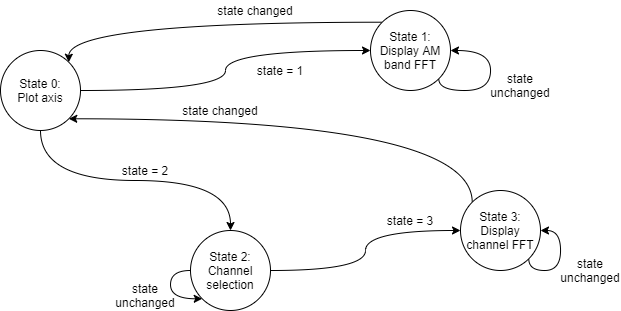
\includegraphics[width=0.75\linewidth]{2021/Images/Design/statediagram.png}
%     \caption{Experimental Setup Overview}
%     \label{fig:expsetup}
% \end{figure}

% \subsection{Band pass IIR Filter using BZT}
% The BZT implementation method is used to implement the digital band pass IIR filter. Using \cite{ETSI} standards for emission levels with channel bandwidth $F=9kHz$, the following is selected for the pass band and stop band frequencies, for all channels with $f_0$ being the center of each channel:
% \begin{align}
%    A_{\pm 0.5 F} &= -3dB \\
%    A_{\pm 0.7 F} &= -35dB \\
%     f_p &= f_0 \pm 4.5kHz \\
%     f_s &= f_0 \pm 6.3kHz
% \end{align}

% From specifications the pre-warped frequencies are:
% \begin{align}
%     \omega`_{p1} &= \tan \left(\frac{2 \pi \times (f_0 - 4.5 \times 10^3)}{2 \times 4.8 \times 10^6} \right)\\
%     \omega`_{p2} &= \tan \left(\frac{2 \pi \times (f_0 + 4.5 \times 10^3)}{2 \times 4.8 \times 10^6} \right)\\
%     \omega`_{s1} &= \tan \left(\frac{2 \pi \times (f_0 - 6.3 \times 10^3)}{2 \times 4.8 \times 10^6} \right)\\
%     \omega`_{s1} &= \tan \left(\frac{2 \pi \times (f_0 + 6.3 \times 10^3)}{2 \times 4.8 \times 10^6} \right) \\
%     \nonumber \\
%     \omega_0^2 &= \omega`_{p1} \omega`_{p2} \\
%     W &= \omega`_{p2} - \omega`_{p1} \\
%     \omega_s^p &= min(\frac{\omega`_{p1}}{\omega`_{s1}}, \frac{\omega`_{p2}}{\omega`_{s2}})
% \end{align}
% Thus the order of the prototype LPF can be obtained, since the audio requirement, a Butterworth filter is used over the Chebyshev implementation. Using above values the maximum of all the different channels is selected, using Python (\ref{Python_Code_Appendix}):
% \begin{align}
%     A_s &= 35dB \\
%     A_p &= 1dB \\
%     N &\geq \frac{\log \left(\frac{10^{\frac{A_s}{10}}}{10^{\frac{A_p}{10}}} - 1\right)}{2 \log \left(\frac{\omega_s^p}{\omega_p^p} \right)} \\
%     N &\geq 11.71
% \end{align}
% Choosing $N = 12$. Thus the s-plane transfer function for the 6th order LP filter is:
% \begin{align}
%     H(s) &= \frac{1}{s^6 + 1}
% \end{align}
% Using the lowpass-to-bandpass transformation:
% \begin{align}
%     H'(s) &= H(s) \Big|_{s=\frac{Ws}{s^2 + \omega_0^2}} \\
%           &= \frac{1}{\left(\frac{Ws}{s^2 + \omega_0^2}\right)^6 + 1} \\
%           &= \frac{\left(s^2+\omega_0^2\right)^6}{W^6s^6+\left(s^2+\omega_0^2\right)^6}
% \end{align}
% Applying the BZT gives:
% \begin{align}
%     H(z) &= H'(s) \Big|_{s=\frac{z-1}{z+1}} \\
%     &= \frac{\left(\frac{z-1}{z+1}^2+\omega_0^2\right)^6}{W^6\frac{z-1}{z+1}^6+\left(\frac{z-1}{z+1}^2+\omega_0^2\right)^6}
% \end{align}

% For further calculations the critical frequencies of the last channel, $f_0 = 1.602MHz$, will be used:
% \begin{align}
%     \omega_{s1} &= 1.72085 \\
%     \omega_{s2} &= 1.75399 \\
%     \omega_{p1} &= 1.72552 \\
%     \omega_{p2} &= 1.74919 \\
%     \omega_0^2 &= 3.018277 \\
%              W &= 0.023670 \\
%     \omega_s^p &= 1.398381 \\
%     \omega_p^p &= 1
% \end{align}


% \pendsign

% \section[2021/06/19]{Saturday, 19 June 2021}
% \subsection{Bandpass filters}
% Using \cite{etsi} standards for emission levels with channel bandwidth $F=9kHz$. The following is selected:
% \begin{align}
%    \pm 0.5 F &= -3dB \\
%    \pm 0.7 F &= -35dB \\
%     f_p &= f_0 \pm 4.5kHz \\
%     f_s &= f_0 \pm 6.3kHz
% \end{align}
% From specifications the prewarped frequencies are:
% \begin{align}
%     \omega`_{p1} &= \tan \left(\frac{2 \pi \times (f_0 - 4.5 \times 10^3)}{2 \times 4.8 \times 10^6} \right)\\
%     \omega`_{p2} &= \tan \left(\frac{2 \pi \times (f_0 + 4.5 \times 10^3)}{2 \times 4.8 \times 10^6} \right)\\
%     \omega`_{s1} &= \tan \left(\frac{2 \pi \times (f_0 - 6.3 \times 10^3)}{2 \times 4.8 \times 10^6} \right)\\
%     \omega`_{s1} &= \tan \left(\frac{2 \pi \times (f_0 + 6.3 \times 10^3)}{2 \times 4.8 \times 10^6} \right) \\
%     \nonumber \\
%     \omega_0^2 &= \omega`_{p1} \omega`_{p2} \\
%     W &= \omega`_{p2} - \omega`_{p1} \\
%     \omega_s^p &= min(\frac{\omega`_{p1}}{\omega`_{s1}}, \frac{\omega`_{p2}}{\omega`_{s2}})
% \end{align}
% Thus the order of the prototype LPF can be obtained, using above values:
% \begin{align}
%     A_s &= 35dB \\
%     A_p &= 1dB \\
%     N &\geq \frac{\log \left(\frac{10^{\frac{A_s}{10}}}{10^{\frac{A_p}{10}}} - 1\right)}{2 \log \left(\frac{\omega_s^p}{\omega_p^p} \right)}
% \end{align}

% \pendsign

% \section[2021/06/22]{Tuesday, 22 June 2021}
% \lstloadlanguages{[Visual]C++,[ISO]C++}.
% \lstinputlisting{Code/BZT1.m}
% \pendsign

% \section[2021/06/22]{Thursday, 24 June 2021}
% \lstinputlisting{Code/BZT.m}

% \section[2021/06/26]{Saturday, 26 June 2021}
% Channels 1 - something coefficients for biquad realisation: \\
% {4.3441030483401e-13, 8.6882204553228e-13, 4.3440542735193e-13, 1.0125999657859, -0.9832121491467, \\
% 1, -2.0000053622024, 1.0000022566955, 1.0203381350262, -0.98325710621944, \\
% 1, 2.0038104454451, 1.0038249843642, 1.0081383512962, -0.98765451665787,\\
% 1, 1.9961862492367, 0.99620077555911, 1.029309512043, -0.98774482906519,\\
% 1, -2.0017595627899, 1.0017626730307, 1.0081814007002, -0.99545754066479, \\
% 1, -1.9982350750077, 0.99823817579891, 1.0371738349499, -0.99550304752171}, \\ \\
% {4.3441030483405e-13, 8.7237901853805e-13, 4.3797844880776e-13, 0.98259865833216, -0.98321303403714, 1, 1.9999680323024, 0.99999031125105, 0.99041468200798, -0.98325622128933, 1, 1.9918406130488, 0.99186276162617, 0.97800234833188, -0.98765629419835, 1, -2.0034799170229, 1.0034839569306, 0.99938782061124, -0.98774305136538, 1, -1.9965257407249, 0.99652976095986, 0.97788770660197, -0.99545843633677, 1, -1.9999943422522, 0.99999837227551, 1.007176749645, -0.99550215180959}, {4.3441030483406e-13, 8.6882203130191e-13, 4.3440356977433e-13, 0.95229629367317, -0.98321390133702, 1, -2.0000030185583, 1.0000002459485, 0.96018784803405, -0.98325535395213, 1, 2.0043316057196, 1.0043503895459, 0.94756666059262, -0.98765803640962, 1, 1.9956651217204, 0.99568389136176, 0.96916003493976, -0.98774130900414, 1, -2.001663568993, 1.0016663440572, 0.94729439808566, -0.99545931420852, 1, -1.9983334124487, 0.99833618248682, 0.97687114870403, -0.99550127390006}, {4.3441030483404e-13, 8.6883145646853e-13, 4.3440777359487e-13, 0.92170215605159, -0.98321475208196, 1, 2.0055368100564, 1.0055676748357, 0.92966689215117, -0.98325450317205, 1, 1.9944382209216, 0.99446894714167, 0.91684061420197, -0.9876597453715, 1, -2.002812770078, 1.0028154119638, 0.93863541332991, -0.98773959990113, 1, -1.9999900559119, 0.99999268386563, 0.9164108485374, -0.99546017532785, 1, -1.9971971740101, 0.9971997879745, 0.94626631529235, -0.99550041274517}, {4.3441030483404e-13, 8.6883366785144e-13, 4.3441220411292e-13, 0.89082561902568, -0.98321558724851, 1, 2.0050531909303, 1.0050789546119, 0.89886116358113, -0.98325366797245, 1, 1.994916749508, 0.99494236084172, 0.88583362409534, -0.98766142304514, 1, -2.003138530344, 1.0031418158513, 0.9078233051599, -0.98773792209469, 1, -1.9999961144793, 0.99999939384513, 0.88524652018884, -0.99546102068279, 1, -1.9968653551767, 0.99686862849659, 0.91537162431658, -0.99549956735678}, {4.3441030483405e-13, 8.6882884269539e-13, 4.3440483733936e-13, 0.8596761426026, -0.98321640775897, 1, -2.0000068779172, 1.0000033965402, 0.8677800988515, -0.98325284743089, 1, 2.005606384481, 1.0056379758817, 0.85455519114562, -0.98766307128284, 1, 1.9943746633275, 0.9944061482929, 0.8767331480107, -0.98773627373207, 1, -2.001862378275, 1.0018658660347, 0.8538109612233, -0.99546185120653, 1, -1.9981307438078, 0.99813421873447, 0.88419653954773, -0.99549873680158}, {4.3441030483405e-13, 8.7270948808743e-13, 4.3831080269963e-13, 0.82826327034478, -0.9832172144859, 1, 1.9999771495965, 1.0000037944448, 0.83643321890038, -0.98325204067472, 1, 1.9910707643777, 0.99109730770669, 0.82301489926158, -0.98766469183697, 1, -2.0028926238754, 1.002895415774, 0.84537446476574, -0.98773465306051, 1, -1.9999942441519, 0.99999702764465, 0.8221138028552, -0.99546266778193, 1, -1.9971131319726, 0.9971159072379, 0.85275061071736, -0.99549792019659}
% \pendsign

% \section[2021/06/28]{Monday, 28 June 2021}

% \lstinputlisting{Code/main.c}
